\documentclass[a4paper,10pt]{article}
\usepackage[utf8]{inputenc}

% increase margins
\usepackage{fullpage}
\usepackage[left=1in,top=1in,right=1in,bottom=1in,headheight=3ex,headsep=3ex]{geometry}

% this puts two lines between paragraphs and no indent
\usepackage[parfill]{parskip}

% set up colors
\usepackage{array, xcolor}
\usepackage{color,hyperref}
\usepackage{graphicx}

\definecolor{torontoblue}{HTML}{00204E}
\definecolor{linkblue}{HTML}{0000FF}

% define hyperlink style
\hypersetup{colorlinks,breaklinks,
            linkcolor=linkblue,urlcolor=linkblue,
            anchorcolor=linkblue,citecolor=linkblue}

%opening
\title{Weekly Journal}
\author{Leila Uy}



\begin{document}

\maketitle

%this is commented out, no need for abstract in  your weekly assignment
% \begin{abstract}
% 
% \end{abstract}

\section{Work Update}

This past week, I focused mainly on reading the assigned material and practicing parallel programming in R. The week was busy with personal 
matters like my friend's wedding and holidays so I was not able to read up on GRASS or thoroughly read the code base as much I hoped to.

\subsection{Parallel programming}

\subsubsection{My Computer Specs and AWS}
One of the first thing that any parallel R tells you to do is call \verb|detectCores(logical = True)| and \verb|detectCores(logical = False)|.
This function should tell the number of available hardware threads and cores. For my computer, I have 4 threads and 2 processors. 
Since I have only 2 cores, I have been very careful on trying small parallel programming tasks on my laptop, but Jishnu and I have 
been discussing and for now we are hoping to test future, bigger code on his computer with smaller sets up data before moving to AWS. 

\subsubsection{R}
I went through \textbf{many} resources for parallel R. Some resources were good and some were bad. One of the main things that I discovered 
is that parallel R will work differently depending on the OS of your computer. For example, I was encountering problems with some functions 
in the parallel package in Windows. The function \verb|mclapply| will not work in parallel because of how workers are managed. In addition, 
a socket cluster and fork cluster are different and forking will only work in a Unix-like system.

\subsubsection{Code Base}
I looked at the code base to get an idea of what it is trying to achieve and the steps it takes to achieve it, but one of the things I 
want to do with the code base in the future is go line-by-line in-depth. From there, I want to create a simple flowchart of the code and 
find the best place to preform parallelism similar to the figure below.
\begin{figure}[h!]
    \caption{Flowchart of a simple parallel process}
    \centering
    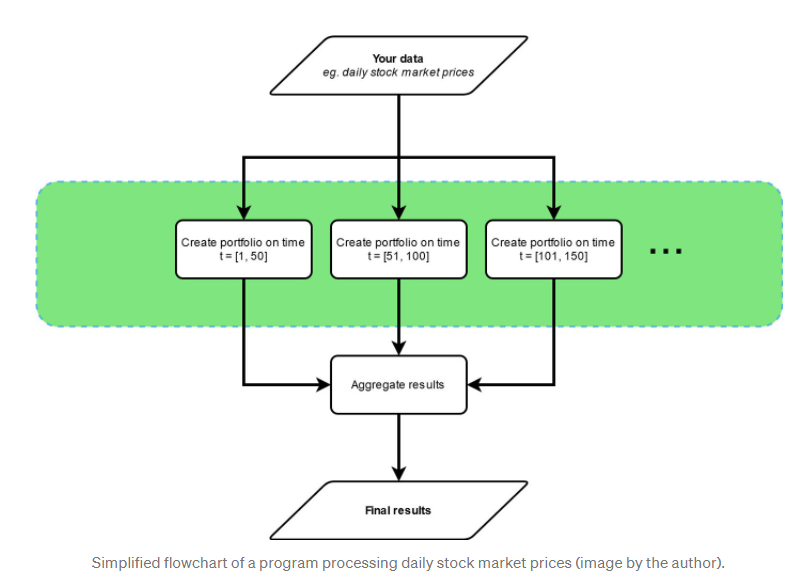
\includegraphics[scale=0.3]{flowchart.png}
\end{figure}

Also, I read about Amdahl's Law which is often used in parallel computing to predict theoretical speedup with multiple processors. I really 
want to try predicting the speedup of parallelization and timing the proces afterwards to see if the prediction was close.

\subsection{Checklist}
So you know my current thought process, this is what I am hoping to look into doing next.
\begin{itemize}
    \item Comment through the code base
    \item Experiment with parallel GRASS with parallel R
    \item Create a flow chart for a parallel version of the code base
    \item Time the serial version of the code base and calculate Amdahl's Law
\end{itemize}

\section{Literature Review}
Aside from the assigned readings, I did not look for other academic journals or publications but mainly blogs/videos/tutorials.

% this info creates the bibliography
% YOU WILL NEED TO CHANGE THIS PATH TO THE LOCATION OF THE BIB file
\bibliography{./agclimate.bib}
\bibliographystyle{plain}


\end{document}
